% !TeX program = pdflatex
% El reloj que nunca suena — un camino verificado a máquina del dilogaritmo a los
% límites de velocidad cuánticos en Lean 4.  Versión española del paper; estructura
% narrativa: cada sección es la pregunta que la produjo.
% Build: pdflatex clock-never-ticks-es.tex  (dos veces, por las referencias)
% Verificado contra el código Lean 2026-06-13 (lake build Dilog QSL, 8426 jobs, exit 0;
% #print axioms en cada teorema -> propext, Classical.choice, Quot.sound).

\documentclass[11pt]{article}
\usepackage[T1]{fontenc}
\usepackage[spanish,es-noshorthands]{babel}
\usepackage{lmodern}
\DeclareUnicodeCharacter{2082}{\ensuremath{_2}}
\DeclareUnicodeCharacter{208A}{\ensuremath{_+}}
\usepackage{amsmath,amssymb,amsthm,booktabs,graphicx,hyperref}
\usepackage{xurl}
\usepackage[table]{xcolor}
\definecolor{ggteal}{HTML}{1B6F8C}
\definecolor{ggband}{HTML}{DCE7EB}
\definecolor{ggamber}{HTML}{E08A1E}
\usepackage[margin=1in]{geometry}
\usepackage{microtype}
\usepackage[most]{tcolorbox}
\usepackage{tikz}
\usetikzlibrary{arrows.meta,positioning}
\setlength{\emergencystretch}{2em}
\graphicspath{{figures/}}
\newtheorem{theorem}{Teorema}
\newtheorem{proposition}{Proposición}
\newtheorem{lemma}{Lema}
\newtheorem{definition}{Definición}
\newtheorem{remark}{Observación}
\newcommand{\lean}[1]{\texttt{#1}}
\newcommand{\R}{\mathbb{R}}
\newcommand{\N}{\mathbb{N}}
\newcommand{\C}{\mathbb{C}}
\newcommand{\Li}{\mathrm{Li}_2}
\newcommand{\Cl}{\mathrm{Cl}_2}
\DeclareMathOperator{\Lrog}{L}
\hypersetup{colorlinks=true,linkcolor=ggteal,citecolor=ggteal,urlcolor=ggteal}
\newtcbox{\keybox}{on line,boxrule=0.9pt,colframe=ggteal,colback=ggband!40,
  arc=3pt,left=8pt,right=8pt,top=5pt,bottom=5pt}
\newcommand{\keyeq}[1]{\begin{center}\keybox{$\displaystyle #1$}\end{center}}
\newtcolorbox{recipebox}[1]{boxrule=0.9pt,colframe=ggamber,colback=ggband!25,
  arc=3pt,title={\textbf{#1}},fonttitle=\small,fontupper=\small}

\title{\bf El reloj que nunca suena\\[4pt]
  \large\normalfont Un camino verificado a m\'aquina del dilogaritmo\\
  a los l\'imites de velocidad cu\'anticos en Lean~4}
\author{Carles Mar\'in\thanks{Formalizado con asistencia de IA (Claude, Anthropic); las
matem\'aticas y todas las afirmaciones son responsabilidad del autor. La metodolog\'ia y
la frontera exacta de la contribuci\'on se discuten en la Secci\'on~\ref{sec:boundary}.}\\[3pt]
  \normalsize Investigador independiente\\
  \normalsize \texttt{karlesmarin@gmail.com}}
\date{Junio 2026}

\begin{document}
\maketitle

\begin{abstract}
El c\'odigo fuente de Mathlib contiene un comentario que se refiere al dilogaritmo
$\Li$ --- una funci\'on que la biblioteca no tiene. Llenamos ese hueco y seguimos las
preguntas hasta donde llevan. El resultado es un desarrollo en Lean~4 sin \lean{sorry}
($\sim$1\,500 l\'ineas sobre Mathlib) que contiene, hasta donde sabemos, varias primicias
en cualquier asistente de demostraci\'on: el dilogaritmo real con la identidad de reflexi\'on
de Euler, la transformaci\'on de Landen, la f\'ormula de duplicaci\'on y la escalera
\'aurea $\Li(1/\varphi^2)=\pi^2/15-\ln^2\varphi$, $\Li(1/\varphi)=\pi^2/10-\ln^2\varphi$
(derivada de un sistema lineal $3\times 3$ --- sin relaci\'on de cinco t\'erminos); el
valor de Rogers $\Lrog(1/\varphi^2)=\pi^2/15$, equivalentemente la carga central
efectiva de Lee--Yang $c_{\mathrm{eff}}=2/5$, la identidad dilogar\'itmica m\'as simple
del ansatz termodin\'amico de Bethe; la funci\'on de Clausen $\Cl$ y la \emph{constante
de Catalan} $G=\Cl(\pi/2)$; la \emph{desigualdad de Fej\'er--Jackson}
$\sum_{k=1}^{M}\sin(k\theta)/k>0$ en $(0,\pi)$; la positividad
$\Cl(\theta)\ge\sin(\theta)/2$ por una sumaci\'on de Abel sin asint\'otica; y los
l\'imites de velocidad cu\'anticos de \emph{Margolus--Levitin} y (en forma $L^1$)
\emph{Mandelstam--Tamm}. Las piezas se ensamblan en el desenlace que promete el
t\'itulo: el estado cu\'antico con poblaciones $\propto 1/n^2$ sobre niveles de
energ\'ia equiespaciados tiene energ\'ia media \emph{infinita} y varianza de energ\'ia
\emph{infinita} --- ambos l\'imites de velocidad de los libros de texto no dicen nada ---
y sin embargo \emph{nunca} alcanza un estado ortogonal a s\'i mismo, porque su
autocorrelaci\'on es $\tfrac{6}{\pi^2}\Li(e^{-i\theta})$ y el dilogaritmo no tiene
ceros en el c\'irculo unidad. Un reloj con presupuesto energ\'etico ilimitado que nunca
suena. Somos exactos con la frontera: cada identidad aqu\'i es cl\'asica (Euler, Landen,
Clausen, Fej\'er, Jackson, Mandelstam--Tamm, Margolus--Levitin); la contribuci\'on es el
desarrollo verificado a m\'aquina y su ensamblaje. Cada teorema depende solo de los tres
axiomas est\'andar.
\end{abstract}

\medskip
\noindent\emph{C\'omo leer este art\'iculo.} Est\'a escrito como la historia de seis
preguntas. Cinco forman una cadena --- cada secci\'on abre con su pregunta y cierra
entregando al lector la siguiente. La sexta (\emph{¿c\'omo de r\'apido puede
evolucionar un estado cu\'antico?}) \emph{no} naci\'o de la cadena: naci\'o por su
cuenta, de preguntar qu\'e parte de la met\'afora «el universo es una computadora» es un
teorema de verdad, y se \emph{cruz\'o} con la cadena al final. La
Figura~\ref{fig:map} es el mapa honesto, cruce incluido. Si solo va a leer una cosa,
lea el Teorema~\ref{thm:clock} y la Figura~\ref{fig:clock}; el inventario Lean es la
Tabla~\ref{tab:inventory}, y reproducirlo todo son tres \'ordenes
(Ap\'endice~\ref{app:repro}).

\begin{figure}[h]
\centering
\begin{tikzpicture}[
  obj/.style={draw=ggteal, thick, rounded corners=2pt, fill=ggband!40,
    align=center, font=\small, inner sep=5pt},
  q/.style={font=\scriptsize\itshape, text=ggamber!80!black, align=center},
  arr/.style={-{Stealth[length=2.4mm]}, thick, ggteal}]
\node[obj] (hole) {un hueco en\\la biblioteca};
\node[obj, right=31mm of hole] (li2) {$\Li$ y sus ecuaciones\\funcionales};
\node[obj, right=31mm of li2] (gold) {la escalera\\\'aurea};
\node[obj, below=16mm of gold] (circle) {el c\'irculo:\\par\'abola $+$ $\Cl$};
\node[obj, left=31mm of circle] (pos) {Fej\'er--Jackson:\\$\Cl>0$};
\node[obj, left=31mm of pos, fill=ggamber!25, draw=ggamber] (clock)
  {\textbf{el reloj que}\\\textbf{nunca suena}};
\node[obj, below=18mm of pos] (qsl) {l\'imites de velocidad:\\Margolus--Levitin,\\Mandelstam--Tamm};
\node[q, below=1mm of qsl] {nacida aparte: «¿qu\'e parte de\\`el universo es una
  computadora' es un teorema?»};
\draw[arr] (hole) -- node[q, above=1.2mm] {P1: ¿qu\'e sabe\\la serie?} (li2);
\draw[arr] (li2) -- node[q, above=1.2mm] {P2: ¿escalera\\sin Abel?} (gold);
\draw[arr] (gold) -- node[q, right=1.5mm] {P3: ¿qu\'e pasa\\en el c\'irculo?} (circle);
\draw[arr] (circle) -- node[q, above=1.2mm] {P4: ¿por qu\'e es positiva\\la mitad salvaje?} (pos);
\draw[arr] (pos) -- node[q, above=1.2mm] {P5: ¿qu\'e cosa f\'isica\\late con esto?} (clock);
\draw[arr] (qsl) -| node[q, left=1mm, pos=0.85] {los hilos\\se cruzan} (clock);
\end{tikzpicture}
\caption{El mapa honesto. El hilo del dilogaritmo recorre la fila de arriba y vuelve;
el hilo cu\'antico (abajo) naci\'o por su cuenta y se \emph{cruz\'o} con \'el al final
--- el cruce, no la cadena, es donde vive el teorema del t\'itulo. Cada nodo es un
bloque de Lean sin \lean{sorry}.}
\label{fig:map}
\end{figure}

\section{La pregunta que lo inicia: ¿por qu\'e la biblioteca cita una funci\'on que no
tiene?}\label{sec:intro}

El archivo \lean{Mathlib/Analysis/SpecialFunctions/Integrals/LogTrigonometric.lean} de
Mathlib --- la biblioteca matem\'atica del asistente de demostraci\'on Lean~4, sobre la que se
construye buena parte de la matem\'atica formalizada contempor\'anea --- describe una de
sus integrales refiri\'endose al dilogaritmo
\[
\Li(x) \;=\; \sum_{n\ge 1}\frac{x^n}{n^2}.
\]
La funci\'on en s\'i no est\'a. Y no solo en Mathlib: hasta donde pudimos determinar, el
dilogaritmo, la funci\'on de Clausen, la constante de Catalan, la desigualdad de
Fej\'er--Jackson y todos los l\'imites de velocidad cu\'anticos est\'an ausentes de
\emph{todos} los asistentes de demostraci\'on (Lean, Rocq/Coq, Isabelle); las bibliotecas
cu\'anticas existentes (CoqQ, SQIR, Isabelle Marries Dirac) formalizan circuitos, no
cotas din\'amicas.\footnote{Comprobaciones de junio de 2026: Loogle y \lean{grep} sobre
Mathlib (cero declaraciones \lean{quantum}; nada de
\lean{dilog}/\lean{polylog}/\lean{Clausen}, y solo \emph{n\'umeros} de Catalan);
b\'usquedas sobre el Archive of Formal Proofs y los ecosistemas Rocq/Coq. Ausencia de
evidencia, con esa cautela.}

¿C\'omo una funci\'on tan central queda sin formalizar durante una d\'ecada de Mathlib?
Porque vive en un punto ciego: demasiado especial para ser infraestructura, demasiado
anal\'itica para ser \'algebra, y custodiada --- como veremos --- por exactamente un
l\'imite genuinamente delicado. La g\'enesis de este proyecto fue una auditor\'ia: una
verificaci\'on num\'erica a cincuenta d\'igitos de las identidades dilogar\'itmicas de
un preprint reciente de Alha~\cite{alha}. Auditar los dilogaritmos de otro nos mand\'o a
la biblioteca a por una implementaci\'on de referencia; la biblioteca nos devolvi\'o con
las manos vac\'ias. Decidimos llenar el hueco y seguir haciendo la siguiente pregunta
hasta que las preguntas se acabaran. Se acabaron cinco secciones despu\'es, dentro de un
problema de mec\'anica cu\'antica. Este art\'iculo es el cuaderno de viaje.

\section{P1: ¿qu\'e sabe la serie de su propia derivada?}\label{sec:dilog}

\emph{Apunte hist\'orico.} La funci\'on es de Euler (1768); la identidad de reflexi\'on
es suya. La transformaci\'on de Landen es de 1780. Todo lo de esta secci\'on es
cl\'asico (Lewin~\cite{lewin}, Zagier~\cite{zagier}); el Lean es
\lean{Dilog/Basic.lean}.

Una serie de potencias se deriva t\'ermino a t\'ermino, y la derivada del dilogaritmo
colapsa a funciones elementales:
\[
\Li'(x) \;=\; \sum_{n\ge1}\frac{x^{n-1}}{n} \;=\; -\frac{\ln(1-x)}{x}
\qquad(\lvert x\rvert<1,\ x\ne 0).
\]
En Lean esta \'unica l\'inea es el coraz\'on anal\'itico de todo el desarrollo ---
derivaci\'on t\'ermino a t\'ermino bajo mayorante geom\'etrica
(\lean{hasDerivAt\_tsum\_of\_isPreconnected}) y la serie de Mercator para identificar la
suma. Conocida la derivada, las ecuaciones funcionales se vuelven mec\'anicas:

\begin{recipebox}{Receta: una ecuaci\'on funcional en tres movimientos}
Para probar que una combinaci\'on $F$ de dilogaritmos y logaritmos es constante en un
intervalo: (1)~derivar t\'ermino a t\'ermino y comprobar $F'=0$ con las reglas de
cadena/producto m\'as \lean{field\_simp; ring}; (2)~concluir que $F$ es constante por la
maquinaria del valor medio (\lean{constant\_of\_has\_deriv\_right\_zero} en
subintervalos); (3)~evaluar la constante como \emph{l\'imite en la frontera}. En el paso
(3) vive el \'unico l\'imite delicado del tema: $\ln x\cdot\ln(1-x)\to 0$ en el extremo,
domado como $\big(\ln(1-x)/x\big)\cdot\big(x\ln x\big)\to(-1)\cdot 0$ v\'ia la
caracterizaci\'on por pendientes de la derivada y
\lean{tendsto\_log\_mul\_rpow\_nhdsGT\_zero}. La continuidad de $\Li$ hasta la frontera
es el criterio $M$ de Weierstrass (\lean{continuousOn\_tsum}).
\end{recipebox}

\begin{theorem}[{\lean{Li₂\_add\_Li₂\_one\_sub}, \lean{Li₂\_landen},
\lean{Li₂\_sq}, \lean{Li₂\_one\_half}}]\label{thm:funceq}
En los dominios indicados,
\begin{align*}
\Li(x)+\Li(1-x) &= \tfrac{\pi^2}{6}-\ln x\,\ln(1-x) && x\in(0,1)\\
\Li(x)+\Li\!\Big(\tfrac{x}{x-1}\Big) &= -\tfrac{1}{2}\ln^2(1-x) && x\in(0,\tfrac12)\\
\Li(x^2) &= 2\big(\Li(x)+\Li(-x)\big) && \lvert x\rvert\le 1\\
\Li(\tfrac12) &= \tfrac{\pi^2}{12}-\tfrac{\ln^2 2}{2}.
\end{align*}
\end{theorem}

Dos notas de honestidad, ambas visibles en los enunciados Lean. El dominio de Landen se
detiene en $x=\frac12$: m\'as all\'a, el argumento $x/(x-1)$ sale del disco de
convergencia, y una definici\'on por serie de potencias no contin\'ua anal\'iticamente
--- y no fingimos que lo haga. Y la f\'ormula de duplicaci\'on no necesita c\'alculo en
absoluto: es un puro reordenamiento de la serie por \'indices pares e impares
(\lean{tsum\_even\_add\_odd}), el espejo formal de c\'omo la habr\'ia probado Euler.

\emph{El giro.} Con tres ecuaciones funcionales en la mano, las joyas cl\'asicas del
tema son las evaluaciones \'aureas --- y todos los libros de texto llegan a ellas por la
relaci\'on de cinco t\'erminos de Abel, una identidad de dos variables que \emph{no}
hemos formalizado. ¿Estamos atascados?

\section{P2: ¿se puede subir la escalera \'aurea sin la relaci\'on de Abel?}
\label{sec:golden}

\emph{Apunte hist\'orico.} Los valores son de Landen (1780); la suma de dos t\'erminos
es de la memoria de Rogers de 1907~\cite{rogers}. Su papel como carga central pertenece
al ansatz termodin\'amico de Bethe de los a\~nos
noventa~\cite{zamolodchikov,nahm,kirillov}.

La respuesta es s\'i, y la llave son dos accidentes aritm\'eticos de la raz\'on \'aurea
$\varphi=(1+\sqrt5)/2$, ambos consecuencia inmediata de $\varphi^2=\varphi+1$:
\[
\frac{1}{\varphi}+\frac{1}{\varphi^2}=1
\qquad\text{y}\qquad
\frac{1/\varphi^2}{1/\varphi^2-1}=-\frac{1}{\varphi}.
\]
El primero dice que $1/\varphi$ y $1/\varphi^2$ son una \emph{pareja de reflexi\'on}; el
segundo, que \emph{Landen lleva $1/\varphi^2$ a $-1/\varphi$} --- y n\'otese que
$1/\varphi^2\approx0.382<\tfrac12$: dentro de nuestro dominio probado de Landen.
Reflexi\'on en $1/\varphi^2$, Landen en $1/\varphi^2$, duplicaci\'on en $1/\varphi$:
tres ecuaciones lineales, tres inc\'ognitas, y \lean{linarith} cierra el sistema.
\keyeq{
\Li\!\Big(\tfrac{1}{\varphi^2}\Big)=\tfrac{\pi^2}{15}-\ln^2\varphi,
\qquad
\Li\!\Big(\tfrac{1}{\varphi}\Big)=\tfrac{\pi^2}{10}-\ln^2\varphi,
\qquad
\Li\!\Big(-\tfrac{1}{\varphi}\Big)=\tfrac{\ln^2\varphi}{2}-\tfrac{\pi^2}{15}.
}
Sin relaci\'on de cinco t\'erminos --- un descubrimiento peque\~no pero grato del proceso
de formalizaci\'on. En la normalizaci\'on de Rogers
$\Lrog(x)=\Li(x)+\tfrac12\ln x\ln(1-x)$ los defectos $\ln^2$ se cancelan
(\lean{rogersL\_inv\_goldenRatio\_sq}, \lean{rogersL\_gold\_sum}):
\[
\Lrog\!\Big(\tfrac{1}{\varphi^2}\Big)=\frac{\pi^2}{15},\qquad
\Lrog\!\Big(\tfrac{1}{\varphi}\Big)+\Lrog\!\Big(\tfrac{1}{\varphi^2}\Big)
=\frac{\pi^2}{6}=\Lrog(1),
\]
y el primero, normalizado, es la carga central efectiva del ansatz de Bethe
termodin\'amico de Lee--Yang, $c_{\mathrm{eff}}=\Lrog(1/\varphi^2)/\Lrog(1)=2/5$ ---
hasta donde sabemos, la primera identidad dilogar\'itmica TBA verificada en un asistente
de pruebas. La Figura~\ref{fig:golden} muestra la curva con sus valores certificados.

\begin{figure}[t]
\centering
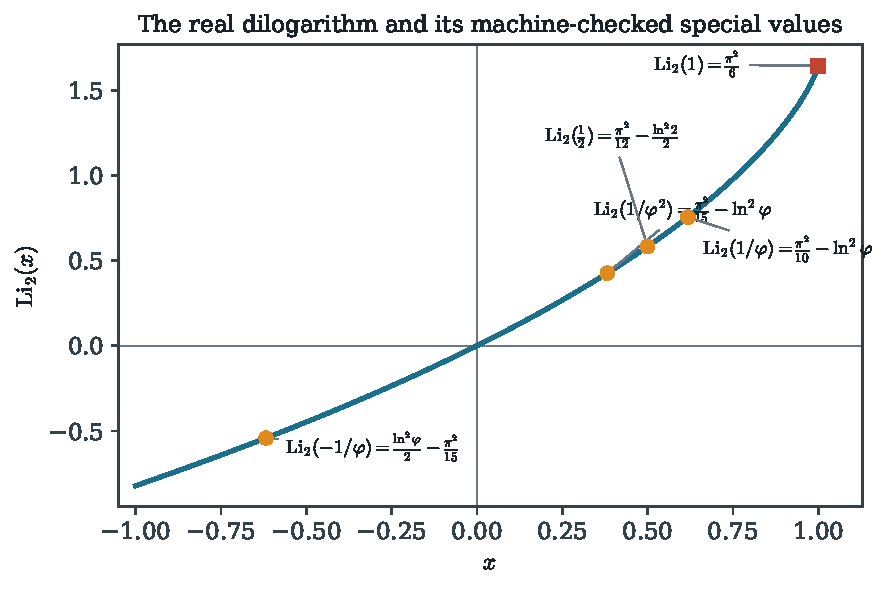
\includegraphics[width=0.78\textwidth]{dilog_fig1_golden}
\caption{El dilogaritmo real. Cada valor marcado es un teorema Lean sin \lean{sorry};
el script generador verifica cada uno contra num\'erica de 40 d\'igitos antes de
dibujar.}
\label{fig:golden}
\end{figure}

\emph{El giro.} La escalera vive la vida de la funci\'on \emph{dentro} del intervalo de
convergencia. El siguiente territorio natural es la propia frontera. ¿Qu\'e hace la
serie en el c\'irculo unidad?

\section{P3: ¿qu\'e pasa en el c\'irculo?}\label{sec:circle}

\emph{Apunte hist\'orico.} Clausen introdujo su funci\'on en 1832~\cite{clausen}; la
constante de Catalan es de su memoria de 1865, y su irracionalidad sigue, famosamente,
abierta. La serie del coseno de abajo es el desarrollo de Fourier del polinomio de
Bernoulli $B_2$, que Mathlib ya posee (\lean{hasSum\_one\_div\_nat\_pow\_mul\_cos}); el
Lean de esta secci\'on es \lean{Dilog/Clausen.lean}.

En el c\'irculo el dilogaritmo se parte en una mitad mansa y una mitad salvaje:
\[
\Li(e^{i\theta}) \;=\;
\underbrace{\sum_{n\ge1}\frac{\cos n\theta}{n^2}}_{\textstyle
  =\;\frac{\pi^2}{6}-\frac{\pi\theta}{2}+\frac{\theta^2}{4}}
\;+\; i\,\underbrace{\sum_{n\ge1}\frac{\sin n\theta}{n^2}}_{\textstyle =\;\Cl(\theta)}
\qquad(\theta\in[0,2\pi]).
\]
La parte real es una \emph{par\'abola elemental} (\lean{hasSum\_cos\_div\_sq}, desde la
maquinaria Bernoulli--Fourier de Mathlib en $k=1$). La parte imaginaria no es elemental
en absoluto: es la \textbf{funci\'on de Clausen}, una funci\'on especial genuinamente
nueva --- la raz\'on de que exista esta secci\'on. En el cuarto de c\'irculo produce una
celebridad:
\[
G \;=\; \Cl\!\Big(\frac{\pi}{2}\Big) \;=\; \sum_{k\ge0}\frac{(-1)^k}{(2k+1)^2}
\;=\;0{,}9159\ldots,
\]
la \textbf{constante de Catalan}, ausente de todos los asistentes de demostraci\'on hasta ahora
(\lean{catalanConst}, \lean{Cl₂\_pi\_div\_two}; la prueba es el mismo reordenamiento
par/impar que la duplicaci\'on --- los senos de \'indice par se anulan, los impares dan
la serie alternada). Las simetr\'ias b\'asicas salen gratis: $\Cl(0)=\Cl(\pi)=0$, $\Cl$
es impar, y $\Cl(2\pi-\theta)=-\Cl(\theta)$.

\emph{El giro.} Dib\'ujese la mitad salvaje (Figura~\ref{fig:clausen}) y una sospecha
domina todo: entre $0$ y $\pi$ la funci\'on parece \emph{positiva}. Dos valores y una
corazonada no son un teorema. ¿Por qu\'e es positiva? La pregunta es m\'as vieja de lo
que parece: es la de Fej\'er, de 1910.

\section{P4: ¿por qu\'e es positiva la mitad salvaje?}\label{sec:fejer}

\emph{Apunte hist\'orico.} Fej\'er plante\'o y prob\'o parcialmente la positividad de
las sumas parciales del seno en 1910; la prueba de Jackson es de
1911~\cite{fejer,jackson}. Es el abuelo de la teor\'ia de sumas trigonom\'etricas
positivas (Vietoris, Askey). El Lean es \lean{Dilog/FejerJackson.lean}.

\begin{theorem}[{\lean{fejerSum\_pos}}]\label{thm:fj}
Para todo $M\ge1$ y $\theta\in(0,\pi)$:
$\displaystyle\sum_{k=1}^{M}\frac{\sin k\theta}{k}>0$.
\end{theorem}

\emph{Caso comprobable a mano.} $M=2$:
$\sin\theta+\tfrac12\sin2\theta=\sin\theta\,(1+\cos\theta)>0$ en $(0,\pi)$. El valor de
la formalizaci\'on est\'a en que esa misma certeza cubre ahora todo $M$.

La prueba es la inducci\'on cl\'asica por m\'inimo interior, con dos toques que merece
la pena registrar. Primero, el n\'ucleo de Dirichlet se maneja
\emph{multiplicativamente} --- sin divisi\'on, sin singularidad evitable:
\[
2\sin\tfrac{\theta}{2}\sum_{k=1}^{M}\cos k\theta
=\sin\!\big((M+\tfrac12)\theta\big)-\sin\tfrac{\theta}{2},
\]
un telescopio de $\sin((k+\tfrac12)\theta)$ v\'ia la identidad producto-a-suma
(\lean{Finset.sum\_range\_sub}). Segundo, en un m\'inimo local interior la ecuaci\'on
cr\'itica $\sin((M+\tfrac12)\theta_0)=\sin(\theta_0/2)$ \emph{factoriza}
(\lean{Real.sin\_sub\_sin}) como
$\sin(M\theta_0/2)\cos((M{+}1)\theta_0/2)=0$, y sus dos ramas fuerzan
\[
\sin(M\theta_0)=0
\qquad\text{o}\qquad
\sin(M\theta_0)=\sin\theta_0>0:
\]
en ambos casos el \'ultimo t\'ermino de la suma es no negativo en el m\'inimo, as\'i que
el valor m\'inimo supera la suma parcial anterior --- positiva por inducci\'on. Los
valores de frontera se anulan; la compacidad cierra.

De Fej\'er--Jackson a la funci\'on de Clausen hay una sumaci\'on de Abel, y aqu\'i la
formalizaci\'on encontr\'o una peque\~na simplificaci\'on: \emph{no hace falta
asint\'otica}. Escribiendo la suma parcial de $(N{+}1)$ t\'erminos de la serie de $\Cl$
en t\'erminos de las sumas de Fej\'er--Jackson $S_M$,
\[
\sum_{n=1}^{N+1}\frac{\sin n\theta}{n^2}
=\frac{S_{N+1}(\theta)}{N+1}
+\sum_{k=1}^{N}S_k(\theta)\Big(\frac{1}{k}-\frac{1}{k+1}\Big),
\]
cada pieza de la derecha es positiva, y el sumando $k=1$ por s\'i solo vale
$\sin(\theta)/2$. Toda suma parcial es por tanto $\ge\sin(\theta)/2$ --- sin cotas de
n\'umeros arm\'onicos, sin estimaciones de cola --- y el l\'imite hereda la cota
(\lean{Cl₂\_pos}):
\keyeq{\Cl(\theta)\;\ge\;\frac{\sin\theta}{2}\;>\;0\qquad(0<\theta<\pi).}

\begin{figure}[t]
\centering
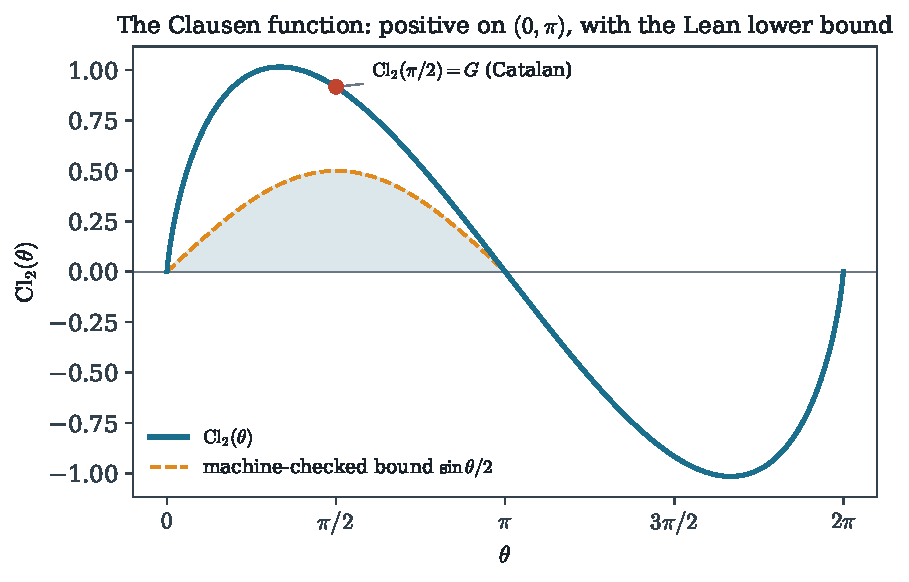
\includegraphics[width=0.78\textwidth]{dilog_fig2_clausen}
\caption{La funci\'on de Clausen en $[0,2\pi]$ con la cota inferior verificada a
m\'aquina $\sin(\theta)/2$ (sombreada) en $(0,\pi)$, y la constante de Catalan en el
cuarto de c\'irculo. El script verifica la cota en una malla de 400 puntos a 30
d\'igitos.}
\label{fig:clausen}
\end{figure}

\emph{El giro --- el grande, y el honesto.} Demos un paso atr\'as y miremos lo que
tenemos en las manos: una suma $\sum p_n e^{-in\theta}$ con pesos positivos
$p_n\propto 1/n^2$, cuya parte imaginaria nunca se anula en $(0,\pi)$. Un f\'isico lee
esa expresi\'on al instante --- es la \emph{autocorrelaci\'on de un estado cu\'antico},
el producto interno entre un estado y su propia evoluci\'on temporal, para poblaciones
$p_n$ sobre niveles de energ\'ia equiespaciados. Debemos ser honestos sobre c\'omo
entr\'o esta lectura en el proyecto, porque \emph{no} naci\'o de la cadena de
preguntas: un hilo paralelo --- nacido de preguntar qu\'e parte de la vieja met\'afora
«el universo es una computadora» es un teorema de verdad --- ya hab\'ia formalizado las
dos cotas cl\'asicas sobre la velocidad de evoluci\'on de cualquier estado cu\'antico.
En este punto los dos hilos se cruzaron: el c\'irculo llevaba todo el tiempo midiendo
\emph{tiempo}, y el teorema de positividad que acab\'abamos de probar era una
afirmaci\'on sobre un sistema cu\'antico que no puede alcanzar un estado ortogonal.
¿Qu\'e dicen sobre \'el los l\'imites de velocidad?

\section{P5: ¿qu\'e cosa f\'isica late con esta funci\'on?}\label{sec:clock}

\emph{Apunte hist\'orico.} Mandelstam y Tamm acotaron el tiempo de ortogonalizaci\'on
por la \emph{dispersi\'on} de energ\'ia en 1945~\cite{mandelstam}; Margolus y Levitin lo
acotaron por la energ\'ia media en 1998~\cite{margolus}. Juntos son los ``l\'imites de
velocidad cu\'anticos'' de los libros de texto: cu\'antos estados distinguibles puede
visitar un sistema por unidad de tiempo, con un presupuesto de energ\'ia dado. El Lean
es \lean{QSL/}.

Un estado $\lvert\psi_0\rangle=\sum_n c_n\lvert E_n\rangle$ evoluciona con
autocorrelaci\'on $S(t)=\sum_n p_n e^{-iE_nt}$, $p_n=\lvert c_n\rvert^2$, y alcanza un
estado ortogonal en el tiempo $\tau$ si y solo si $S(\tau)=0$. Esto es una afirmaci\'on
sobre una funci\'on escalar de una medida espectral discreta no negativa, y as\'i lo
formalizamos --- el espacio de Hilbert es pura contabilidad. La ortogonalidad entra como dos
condiciones reales ($\operatorname{Re}S=\operatorname{Im}S=0$); Margolus--Levitin no
necesita n\'umeros complejos en absoluto.

\begin{theorem}[{\lean{margolus\_levitin}, \lean{mandelstam\_tamm\_L1}}; $\hbar=1$]
\label{thm:qsl}
Si $S(\tau)=0$ con $\tau\ge0$, entonces
\[
\pi \;\le\; 2\,\langle E\rangle\,\tau
\qquad\text{y}\qquad
1 \;\le\; D_1\,\tau,
\quad D_1=\textstyle\sum_n p_n\lvert E_n-\bar E\rvert .
\]
\end{theorem}

El coraz\'on de Margolus--Levitin es una desigualdad de inter\'es independiente,
$\cos x\ge 1-\tfrac{2}{\pi}(x+\sin x)$ para $x\ge0$ (con igualdad en $0$ \emph{y} en
$\pi$), que probamos con el mismo patr\'on unimodal que Fej\'er--Jackson: sube y baja,
ambos extremos en cero, partida en $x_0=2\arctan(2/\pi)$. La misma forma de prueba
carg\'o con tres teoremas de este art\'iculo --- no es casualidad sino t\'ecnica
transferible. Como $D_1\le\Delta E$ por Cauchy--Schwarz, la segunda cota implica la
Mandelstam--Tamm d\'ebil de los libros, $\tau\ge1/\Delta E$; la constante exacta $\pi/2$
necesita el argumento geod\'esico y queda como camino (\S\ref{sec:roads}).

Y ahora el desenlace. T\'omense poblaciones $p_n=\frac{6}{\pi^2 n^2}$ sobre niveles
$E_n=n$: el \emph{estado zeta de peso 2}. Su autocorrelaci\'on \emph{es} nuestra
protagonista,
\[
S(\theta)=\frac{6}{\pi^2}\,\Li(e^{-i\theta})
=\frac{6}{\pi^2}\Big(
\underbrace{\tfrac{\pi^2}{6}-\tfrac{\pi\theta}{2}+\tfrac{\theta^2}{4}}_{\text{la
par\'abola de la \S\ref{sec:circle}}}
\;-\;i\,\underbrace{\Cl(\theta)}_{\text{positiva, por la \S\ref{sec:fejer}}}\Big).
\]
Su energ\'ia media $\sum_n p_n\,n$ \emph{diverge}. Su varianza de energ\'ia tambi\'en.
Ambas cotas del Teorema~\ref{thm:qsl} se cumplen por vacuidad: sobre este estado, los
l\'imites de velocidad de la mec\'anica cu\'antica no predicen nada. Uno podr\'ia
suponer que un estado as\'i, sin cota de energ\'ia, se ortogonaliza al instante. La
verdad es el extremo opuesto:

\begin{theorem}[{\lean{zetaState\_never\_orthogonal}}]\label{thm:clock}
Para todo $\theta\in(0,2\pi)$, las partes real e imaginaria de la autocorrelaci\'on del
estado zeta de peso 2 no son ambas cero: el estado \emph{nunca} alcanza un estado
ortogonal.
\end{theorem}

\begin{proof}[Prueba (tal como en Lean)]
En $(0,\pi)$ la parte imaginaria es $-\Cl(\theta)\ne0$ por la cota de Fej\'er--Jackson.
En $\theta=\pi$ la parte real es el valor de la par\'abola, $-\pi^2/12\ne0$ (es
$-\eta(2)$). En $(\pi,2\pi)$, la reflexi\'on $\Cl(2\pi-\theta)=-\Cl(\theta)$ devuelve el
signo al primer caso.
\end{proof}

De hecho $\lvert S\rvert\ge\frac{6}{\pi^2}\cdot\frac{\pi^2}{12}=\frac12$ en todo el
c\'irculo (certificado num\'ericamente en malla fina; el teorema Lean es la no anulaci\'on): el estado nunca llega ni a \emph{mitad} de camino de la distinguibilidad
(Figura~\ref{fig:clock}). Un reloj con presupuesto energ\'etico infinito cuya campana
nunca llega a sonar --- porque el presupuesto se gasta en una cola espectral
pesada y no en separaci\'on coherente. La energ\'ia es necesaria para la velocidad de
evoluci\'on (Margolus--Levitin); este es el contrapunto verificado a m\'aquina de que no
es, ni de lejos, suficiente.

\begin{figure}[t]
\centering
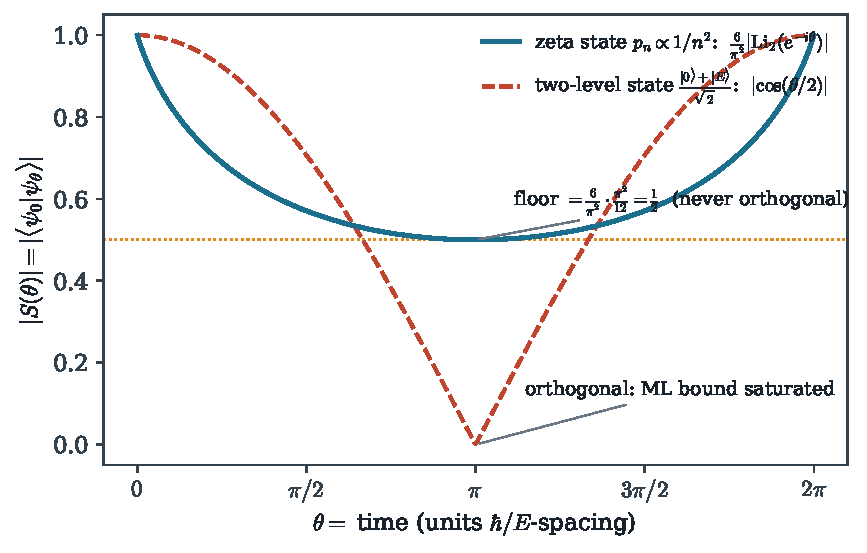
\includegraphics[width=0.82\textwidth]{dilog_fig3_clock}
\caption{Dos estados con el mismo espaciado de niveles. El estado de dos niveles
$(\lvert0\rangle+\lvert2E\rangle)/\sqrt2$ (discontinuo) satura Margolus--Levitin y
alcanza la ortogonalidad en $\theta=\pi$. El estado zeta (continuo), con energ\'ia media
\emph{infinita}, tiene $\lvert S\rvert\ge\frac12$: el reloj que nunca suena. El script
verifica que el suelo vale $\eta(2)=\pi^2/12$ en $\theta=\pi$.}
\label{fig:clock}
\end{figure}

\begin{remark}[Qu\'e relojes s\'i suenan: una observaci\'on de cierre]\label{rem:ek}
Para poblaciones mon\'otonas no crecientes sobre niveles equiespaciados, sonar
(ortogonalizarse) significa un cero de la serie de potencias $\sum_n p_nz^n$ \emph{en}
el c\'irculo unidad --- y el teorema de Enestr\"om--Kakeya (1893/1912)~\cite{enestrom}
localiza esos ceros: ocurren solo en los casos de igualdad, donde los decrementos
$p_{n-1}-p_n$ se concentran en una progresi\'on aritm\'etica, colocando los ceros en
ra\'ices de la unidad. El estado que satura Margolus--Levitin,
$(\lvert0\rangle+\lvert2E\rangle)/\sqrt2$, es exactamente un caso de igualdad
($\frac12(1+z)$, cero en $z=-1$). No hemos encontrado este diccionario --- localizaci\'on
de ra\'ices de polinomios de coeficientes positivos $\leftrightarrow$
ortogonalizabilidad de estados cu\'anticos mon\'otonos --- en ninguna de las dos
literaturas; lo registramos como observaci\'on y como camino.
\end{remark}

\section{La frontera de la contribuci\'on}\label{sec:boundary}

Todo lo que aqu\'i es matem\'atica es cl\'asico: Euler (1768), Landen (1780), Clausen
(1832), Rogers (1907), Fej\'er (1910), Jackson (1911), Mandelstam--Tamm (1945),
Margolus--Levitin (1998); la lectura TBA de los valores \'aureos es de los noventa. No
reclamamos ninguna identidad nueva ni ninguna desigualdad nueva. Las contribuciones son:
(i)~el desarrollo verificado a m\'aquina en s\'i --- seg\'un nuestras comprobaciones de
junio de 2026, la primera formalizaci\'on en cualquier asistente de demostraci\'on de cada
elemento listado en el resumen;
(ii)~tres decisiones de ingenier\'ia de pruebas quiz\'a reutilizables: el telescopio de
Dirichlet sin divisi\'on, la cota de Abel sin asint\'otica $\Cl\ge\sin(\theta)/2$, y los
enunciados completamente reales (medida espectral escalar) de los l\'imites de
velocidad;
(iii)~el ensamblaje del Teorema~\ref{thm:clock}, cuya lectura f\'isica no hemos visto
enunciada, aunque no nos sorprender\'ia que fuera folclore entre especialistas en
polilogaritmos o en QSL; y (iv)~la Observaci\'on~\ref{rem:ek}.

Sobre la metodolog\'ia: la formalizaci\'on se llev\'o a cabo en colaboraci\'on con un
asistente de IA (Claude, Anthropic), con cada paso custodiado por el n\'ucleo de Lean,
cada identidad verificada independientemente a 20--50 d\'igitos \emph{antes} de
formalizar, y cada teorema comprobado con \lean{\#print axioms} para depender solo de
\lean{propext}, \lean{Classical.choice}, \lean{Quot.sound}. Las matem\'aticas, los
errores y las afirmaciones siguen siendo responsabilidad del autor.

\section{Caminos abiertos}\label{sec:roads}

\begin{enumerate}
\item \textbf{La relaci\'on de cinco t\'erminos de Abel} --- la clave de b\'oveda del
peso 2; con ella, toda identidad dilogar\'itmica de dos variables se sigue. Nuestra
maquinaria de reflexi\'on/Landen es el calentamiento.
\item \textbf{El dilogaritmo complejo} y la funci\'on de Bloch--Wigner; con ellos, la
entrop\'ia de d\'imeros 2D ($G/\pi$ --- Catalan otra vez) y los vol\'umenes
hiperb\'olicos quedan al alcance.
\item \textbf{Mandelstam--Tamm exacta} ($\pi/2\Delta E$, el argumento geod\'esico) y la
cota de Margolus--Levitin para fidelidad arbitraria --- conjeturada en 2003, probada
solo en 2023~\cite{hornedal}: un teorema fresco que formalizar.
\item \textbf{Enestr\"om--Kakeya}, como objetivo de formalizaci\'on y como diccionario
de la Observaci\'on~\ref{rem:ek}.
\item \textbf{Sumas trigonom\'etricas positivas m\'as all\'a de Fej\'er--Jackson}
(Vietoris) --- el kit ya est\'a en su sitio.
\end{enumerate}

\section*{Preguntas para llevarse}

Un art\'iculo construido a base de preguntas debe terminar con las que no supo
responder --- una por estaci\'on del mapa, ninguna ret\'orica.

\begin{enumerate}
\item[\textbf{Sobre P1.}] El peso 1 (logaritmos) no necesita l\'imites delicados; el
peso 2 necesit\'o exactamente uno ($\ln x\cdot\ln(1-x)\to0$, el \'unico sitio donde
nuestra formalizaci\'on tuvo que pelear). ¿Es el n\'umero de l\'imites de frontera
genuinamente delicados un \emph{invariante del peso} --- y qu\'e cuenta?

\item[\textbf{Sobre P2.}] Llegamos a los valores \'aureos de Landen sustituyendo una
identidad de dos variables (la de Abel) por tres de una variable, porque el punto
\'aureo vive donde las \'orbitas de la reflexi\'on y de Landen se cortan. ¿Qu\'e
especializaciones de la relaci\'on de cinco t\'erminos son alcanzables as\'i ---
precisamente: cu\'al es el subgrupo de relaciones generado por reflexi\'on, Landen y
duplicaci\'on dentro del grupo completo de ecuaciones funcionales de $\Li$, y est\'a la
relaci\'on de cinco t\'erminos en \'el?

\item[\textbf{Sobre P3.}] En el c\'irculo, la serie del coseno de peso par es un
polinomio y la del seno es transcendentalmente nueva; en peso impar los papeles se
intercambian. ¿Qu\'e \emph{sabe} la paridad del peso sobre la frontera para
intercambiar la mitad mansa y la salvaje?

\item[\textbf{Sobre P4.}] Tres pruebas de positividad de este desarrollo comparten una
misma forma: sube-y-baja con ambos extremos en cero (Fej\'er--Jackson, la desigualdad
del coseno de Margolus--Levitin, y la propia $\Cl$ v\'ia la integral de
$-\ln(2\sin(t/2))$). ¿Hay un solo teorema detr\'as --- un principio del m\'aximo para
sumas positivas --- del que las tres sean instancias, y ser\'ia \emph{ese} lo correcto
a formalizar a continuaci\'on?

\item[\textbf{Sobre P5.}] El estado zeta derrota a ambos l\'imites de velocidad de los
libros de texto mediante una cola espectral pesada, y sin embargo su comportamiento de
ortogonalizaci\'on est\'a perfectamente determinado. ¿Cu\'al es el funcional correcto
de la medida espectral que \emph{s\'i} decide $\tau_\perp$ --- y es el diccionario de
Enestr\"om--Kakeya de la Observaci\'on~\ref{rem:ek} su sombra sobre los estados
mon\'otonos?

\item[\textbf{Sobre el cruce.}] El teorema del t\'itulo existe porque dos hilos
formalizados se encontraron en un objeto que no era de ninguno. Las bibliotecas de
pruebas de hoy contienen miles de teoremas desconectados. ¿Cu\'antas otras parejas
est\'an a una sustituci\'on de distancia de un Teorema~\ref{thm:clock} --- y
podr\'ia hacerse que un asistente de demostraci\'on \emph{buscara} esos cruces, en vez
de esperarlos?
\end{enumerate}

\appendix

\section{Reproducir}\label{app:repro}

\begin{verbatim}
git clone https://github.com/karlesmarin/godsil-gutman-lean
cd godsil-gutman-lean && lake exe cache get
lake build Dilog QSL
\end{verbatim}
Toolchain de Lean \lean{v4.30.0-rc2}, Mathlib fijada en \lean{701fb6e9}. Las figuras se
regeneran con \lean{python figures/dilog\_fig*.py}; cada script verifica su contenido
matem\'atico contra num\'erica de 20--40 d\'igitos antes de dibujar.

\section{Inventario Lean}

\begin{table}[h]
\centering\small
\begin{tabular}{@{}llr@{}}
\toprule
\rowcolor{ggteal!18} Archivo & Contenido & L\'ineas\\
\midrule
\rowcolor{ggband!35} \lean{Dilog/Basic.lean} & $\Li$: serie, derivada, reflexi\'on, Landen,&\\
\rowcolor{ggband!35} & duplicaci\'on, $\Li(\frac12)$, escalera \'aurea, Rogers $\Lrog$, Lee--Yang & 581\\
\lean{Dilog/Clausen.lean} & $\Cl$, $G$ de Catalan, par\'abola de Bernoulli,
$\Cl\ge\sin\theta/2$,&\\
& $\Cl(2\pi-\theta)=-\Cl(\theta)$, Teorema~\ref{thm:clock} & 332\\
\rowcolor{ggband!35} \lean{Dilog/FejerJackson.lean} & desigualdad de Fej\'er--Jackson & 189\\
\lean{QSL/Basic.lean} & Margolus--Levitin (+ la desigualdad del coseno) & 238\\
\rowcolor{ggband!35} \lean{QSL/MandelstamTamm.lean} & Mandelstam--Tamm, forma $L^1$ & 134\\
\midrule
&& 1\,474\\
\bottomrule
\end{tabular}
\caption{El desarrollo. Todos los teoremas sin \lean{sorry}; axiomas:
\lean{propext}, \lean{Classical.choice}, \lean{Quot.sound} en todo.}
\label{tab:inventory}
\end{table}

\begin{thebibliography}{99}\small
\bibitem{lewin} L.~Lewin, \emph{Polylogarithms and Associated Functions}, North-Holland,
1981.
\bibitem{zagier} D.~Zagier, The dilogarithm function, en \emph{Frontiers in Number
Theory, Physics, and Geometry II}, Springer, 2007.
\bibitem{clausen} T.~Clausen, \"Uber die Function $\sin\varphi+\frac{1}{2^2}\sin2\varphi
+\frac{1}{3^2}\sin3\varphi+$ etc., \emph{J.\ Reine Angew.\ Math.} \textbf{8} (1832).
\bibitem{rogers} L.~J.~Rogers, On function sum theorems connected with the series
$\sum x^n/n^2$, \emph{Proc.\ London Math.\ Soc.} \textbf{4} (1907).
\bibitem{fejer} L.~Fej\'er, Lebesguesche Konstanten und divergente Fourierreihen,
\emph{J.\ Reine Angew.\ Math.} \textbf{138} (1910).
\bibitem{jackson} D.~Jackson, \"Uber eine trigonometrische Summe, \emph{Rend.\ Circ.\
Mat.\ Palermo} \textbf{32} (1911).
\bibitem{mandelstam} L.~Mandelstam e I.~Tamm, The uncertainty relation between energy
and time in nonrelativistic quantum mechanics, \emph{J.\ Phys.\ (USSR)} \textbf{9}
(1945) 249.
\bibitem{margolus} N.~Margolus y L.~B.~Levitin, The maximum speed of dynamical
evolution, \emph{Physica D} \textbf{120} (1998) 188; arXiv:quant-ph/9710043.
\bibitem{zamolodchikov} Al.~B.~Zamolodchikov, Thermodynamic Bethe ansatz in relativistic
models, \emph{Nucl.\ Phys.\ B} \textbf{342} (1990) 695.
\bibitem{nahm} W.~Nahm, Conformal field theory and torsion elements of the Bloch group,
en \emph{Frontiers in Number Theory, Physics, and Geometry II}, Springer, 2007.
\bibitem{kirillov} A.~N.~Kirillov, Dilogarithm identities, \emph{Prog.\ Theor.\ Phys.\
Suppl.} \textbf{118} (1995) 61.
\bibitem{enestrom} G.~Enestr\"om, \emph{\"Ofv.\ af Kungl.\ Vetenskaps-Akad.\ F\"orh.}
\textbf{50} (1893); S.~Kakeya, On the limits of the roots of an algebraic equation with
positive coefficients, \emph{T\^ohoku Math.\ J.} \textbf{2} (1912) 140.
\bibitem{hornedal} N.~H\"ornedal y O.~S\"onnerborn, The Margolus--Levitin quantum
speed limit for an arbitrary fidelity, \emph{Phys.\ Rev.\ Research} \textbf{5} (2023);
v\'ease tambi\'en la prueba elemental en arXiv:2307.16854.
\bibitem{alha} L.~Alha, Families of self-inverse functions and dilogarithm identities,
arXiv:2509.07598.
\bibitem{mathlib} The mathlib Community, The Lean mathematical library, \emph{CPP 2020}.
\end{thebibliography}

\end{document}
